\item Os pinos em $A$ e $B$ estão restritos a se deslocarem nos trilhos vertical e horizontal. Se o braço ranhurado
está fazendo com que a se desloque para baixo em $v_{A}$, determine a velocidade de $B$ como uma função de $\theta$.

\import{../answers/}{answer-5}

\vspace{-1.8cm}
\begin{flushright}
	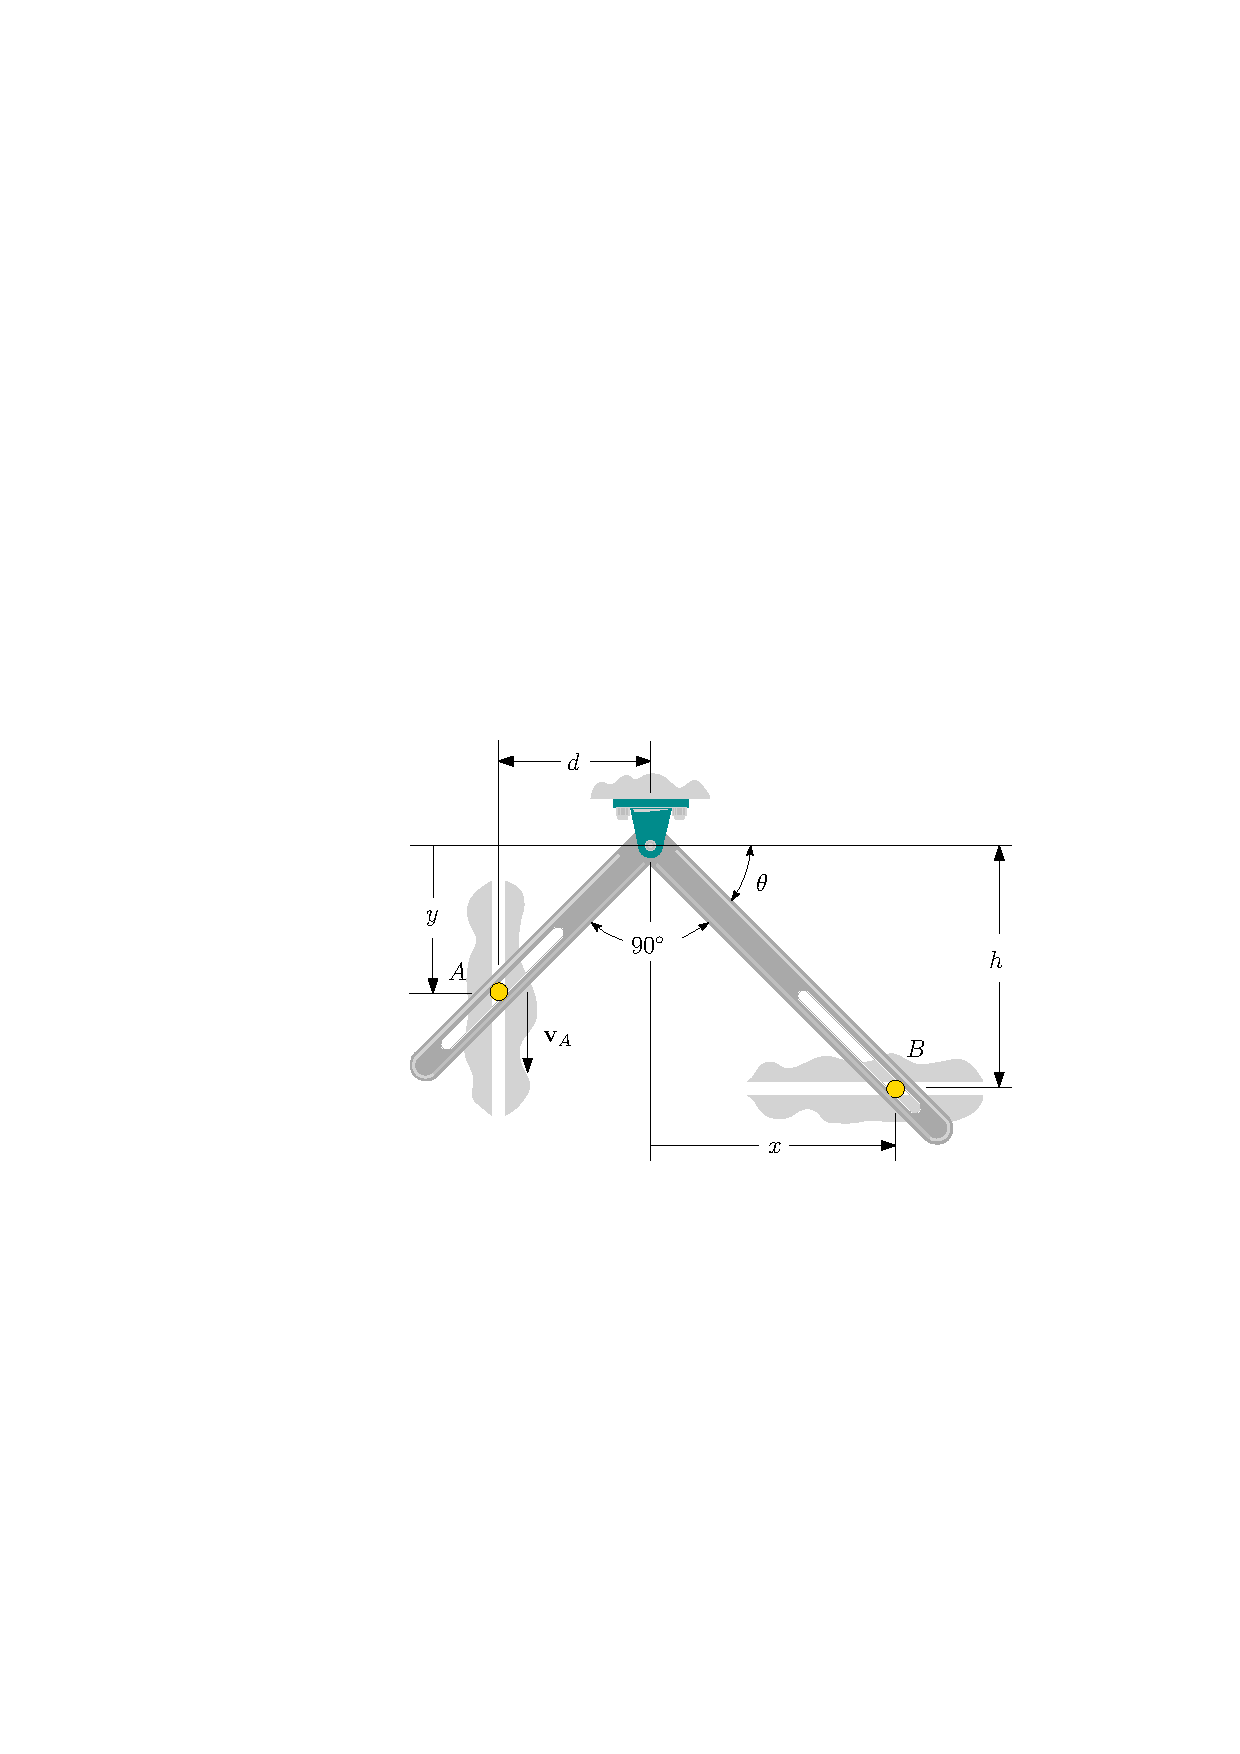
\includegraphics[scale=1]{images/draw_9}
\end{flushright}